\section{Example 1}

Ví dụ này dùng K-means cho tệp dữ liệu ngẫu nhiên 2 chiều (\texttt{k-means-ex1-103.py}). 
Với $K=3$, thuật toán lặp lại hai bước: gán mỗi
điểm cho tâm gần nhất theo khoảng cách Euclid và cập nhật mỗi tâm bằng trung
bình các điểm được gán vào cụm đó. Mục tiêu là giảm tổng bình phương khoảng
cách trong các cụm:
\begin{equation}
    J = \sum_{i=1}^{1500}\left\|\mathbf{x}_i-\boldsymbol{\mu}_{z_i}\right\|_2^2,
    \qquad z_i\in\{0,1,2\}.
\end{equation}
Ở đây $\mathbf{x}_i$ là một điểm dữ liệu, $z_i$ là nhãn cụm và
$\boldsymbol{\mu}_{z_i}$ là tâm của cụm tương ứng.

\subsection{Block 1: Tạo tập dữ liệu}
Ba nhóm điểm được lấy mẫu từ
phân phối chuẩn hai chiều, cùng ma trận hiệp phương sai đơn vị và có trung
bình lần lượt là $(2,2)$, $(8,3)$, $(3,6)$. Mỗi nhóm gồm $N=500$ điểm; sau khi
ghép, ma trận $X$ có kích thước $(1500,2)$ và số cụm cần tìm là $K=3$.

\lstinputlisting[
  firstline=5,
  lastline=19,
  firstnumber=5,
  caption={Sinh ba nhóm dữ liệu và chọn số cụm.},
  label={lst:kmeans-data}
]{../src/k-means-ex1-103.py}

\begin{figure}[htbp]
    \centering
    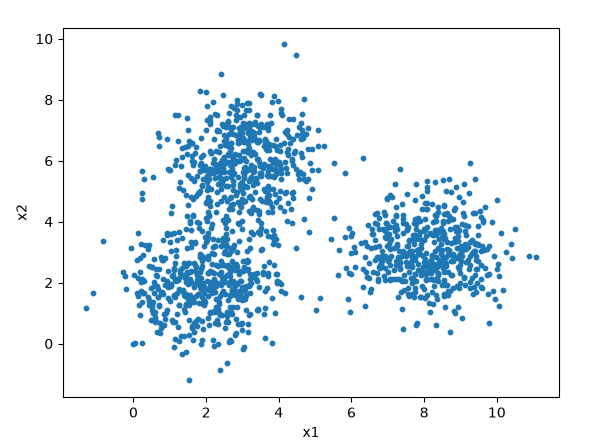
\includegraphics[width=0.52\textwidth]{dataset.png}
    \caption{Tập dữ liệu gồm 1500 điểm trước khi phân cụm.}
    \label{fig:kmeans-data}
\end{figure}

Hình~\ref{fig:kmeans-data} cho thấy ba vùng điểm tập trung quanh các trung
bình đã chọn, đồng thời có một số điểm ở rìa các vùng nằm gần nhau.

\subsection{Block 2: Khởi tạo và gán nhãn}

Ba hàng khác nhau của $X$ được chọn ngẫu nhiên làm tâm ban đầu
. Với mỗi điểm $\mathbf{x}_i$, hàm
\texttt{kmeans\_assign\_labels} dùng \texttt{cdist} để tính khoảng cách đến
từng tâm, rồi lấy chỉ số của tâm gần nhất:
\begin{equation}
    z_i=\operatorname*{arg\,min}_{k\in\{0,1,2\}}
    \left\|\mathbf{x}_i-\boldsymbol{\mu}_k\right\|_2.
\end{equation}
Mảng nhãn trả về có 1500 phần tử, mỗi phần tử nhận một giá trị từ 0 đến 2.

\lstinputlisting[
  firstline=38,
  lastline=55,
  firstnumber=38,
  caption={Chọn tâm ban đầu và gán điểm cho tâm gần nhất.},
  label={lst:kmeans-assign}
]{../src/k-means-ex1-103.py}

\subsection{Block 3: Cập nhật tâm và kiểm tra hội tụ}

Sau khi gán nhãn, tâm cụm $k$ được thay bằng trung bình của các điểm thuộc
cụm đó:
\begin{equation}
    \boldsymbol{\mu}_k^{\mathrm{new}}=
    \frac{1}{|C_k|}\sum_{i\in C_k}\mathbf{x}_i,
    \qquad C_k=\{i:z_i=k\}.
\end{equation}
Hàm \texttt{has\_converged} so sánh tập các tâm cũ và mới; vòng lặp dừng
khi chúng bằng nhau. Cách kiểm tra này dùng giá trị dấu phẩy động đúng bằng
nhau và không có ngưỡng sai số. Hàm cập nhật cũng giả định mỗi cụm đều có
ít nhất một điểm, vì trung bình của cụm rỗng không được xử lý riêng.

\lstinputlisting[
  firstline=59,
  lastline=83,
  firstnumber=59,
  caption={Tính tâm mới và xác định điều kiện dừng.},
  label={lst:kmeans-update}
]{../src/k-means-ex1-103.py}

\subsection{Block 4: Vòng lặp K-means}

Hàm \texttt{kmeans} lưu các tâm và nhãn theo từng bước. Mỗi vòng lặp gán lại
nhãn, tính tâm mới và kiểm tra hội tụ. Biến \texttt{it} chỉ tăng khi tâm mới
khác tâm trước đó; vì vậy số được in ra là số lần cập nhật tâm, không tính
lượt kiểm tra cuối cùng khi thuật toán dừng.

\lstinputlisting[
  firstline=87,
  lastline=98,
  firstnumber=87,
  caption={Vòng lặp gán nhãn, cập nhật tâm và dừng khi hội tụ.},
  label={lst:kmeans-loop}
]{../src/k-means-ex1-103.py}

\subsection{Block 5: Kết quả thực nghiệm}

Code vẽ các điểm theo nhãn cuối cùng và đánh dấu ba tâm bằng các
chấm lớn. 

Kết quả chạy là
\texttt{Number of iterations: 7}; các tâm cuối cùng theo thứ tự nhãn do
chương trình trả về là:
\begin{equation}
\begin{aligned}
    \boldsymbol{\mu}_0 &\approx (1.9835,\;1.9659),\\
    \boldsymbol{\mu}_1 &\approx (3.0270,\;5.9569),\\
    \boldsymbol{\mu}_2 &\approx (8.0748,\;3.0149).
\end{aligned}
\end{equation}
Các tâm này gần với ba trung bình dùng để sinh dữ liệu. Chỉ số nhãn cụm
phụ thuộc vào thứ tự khởi tạo và không mang ý nghĩa thứ bậc.

\lstinputlisting[
  firstline=102,
  lastline=121,
  firstnumber=102,
  caption={Hiển thị nhãn cụm, in số lần cập nhật và các tâm cuối.},
  label={lst:kmeans-result}
]{../src/k-means-ex1-103.py}

\begin{figure}[htbp]
    \centering
    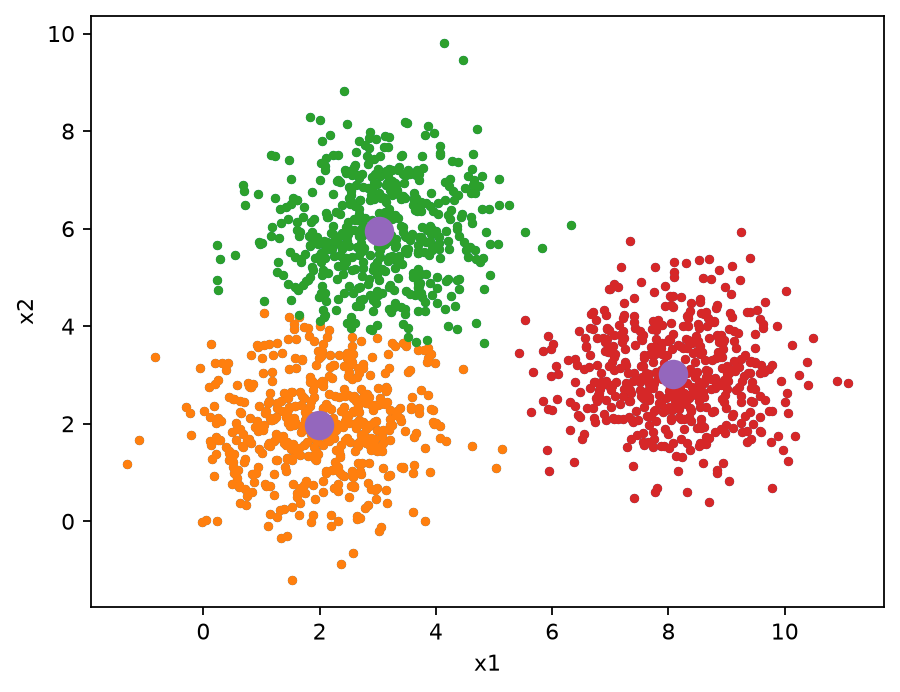
\includegraphics[width=0.62\textwidth]{kmeans_result.png}
    \caption{Kết quả K-means: màu biểu thị nhãn cụm, chấm lớn biểu thị tâm cụm.}
    \label{fig:kmeans-result}
\end{figure}

Hình~\ref{fig:kmeans-result} cho thấy ba cụm tương ứng với ba vùng dữ liệu
ban đầu. Những điểm nằm ở vùng giao nhau được xếp vào cụm có tâm gần nhất,
đúng với quy tắc gán nhãn của thuật toán.

\subsection{So sánh với việc dùng thư viện Scikit-learn}

Để kiểm tra kết quả, file \texttt{k-means-scikit\_learn.py} chạy lại chương trình
lấy đúng ma trận $X$ như file \texttt{k-means-ex1-103.py}, sau đó phân cụm cùng dữ liệu bằng
\texttt{sklearn.cluster.KMeans} với $K=3$, \texttt{random\_state=0},
\texttt{n\_init=10} và \texttt{tol=0}. Trước khi so sánh, chương trình ghép các
tâm gần nhau vì số thứ tự nhãn cụm của hai cách chạy có thể khác nhau. Sau
khi ghép, ba tâm do Scikit-learn trả về lần lượt là
$(1.983497,\,1.965881)$, $(3.027029,\,5.956861)$ và
$(8.074769,\,3.014949)$, kết quả gần như trùng với code ban đầu
đến sáu chữ số thập phân.

\begin{table}[htbp]
    \centering
    \small
    \begin{tabular}{lcc}
        \toprule
        \textbf{Chỉ tiêu} & \textbf{Tự cài đặt} & \textbf{Scikit-learn} \\
        \midrule
        Số lần lặp được báo cáo & 7 & 6 \\
        Inertia & 3005.97947721704 & 3005.9794772170408 \\
        \bottomrule
    \end{tabular}
    \caption{Kết quả hai cách chạy K-means trên cùng 1500 điểm dữ liệu.}
    \label{tab:kmeans-comparison}
\end{table}

Cả $1500/1500$ nhãn đều khớp sau khi ghép nhãn; chỉ số Adjusted Rand bằng
$1.0$. Hai giá trị inertia trong Bảng~\ref{tab:kmeans-comparison} chỉ khác
ở sai số làm tròn dấu phẩy động. 

Số lần lặp $7$ và $6$ không so sánh trực tiếp
được: file tự code đếm số lần tâm thay đổi, còn Scikit-learn báo số vòng
lặp của lần chạy được chọn trong các lần khởi tạo. 

Hai cách cũng khởi tạo tâm khác nhau, file tự code chọn ba điểm ngẫu nhiên từ dữ liệu, còn Scikit-learn chọn ba điểm ngẫu nhiên từ một tập con gồm 10 lần khởi tạo (K-means++).
Nhưng đã hội tụ đến cùng kết quả phân cụm trong ví dụ này.

\begin{figure}[htbp]
    \centering
    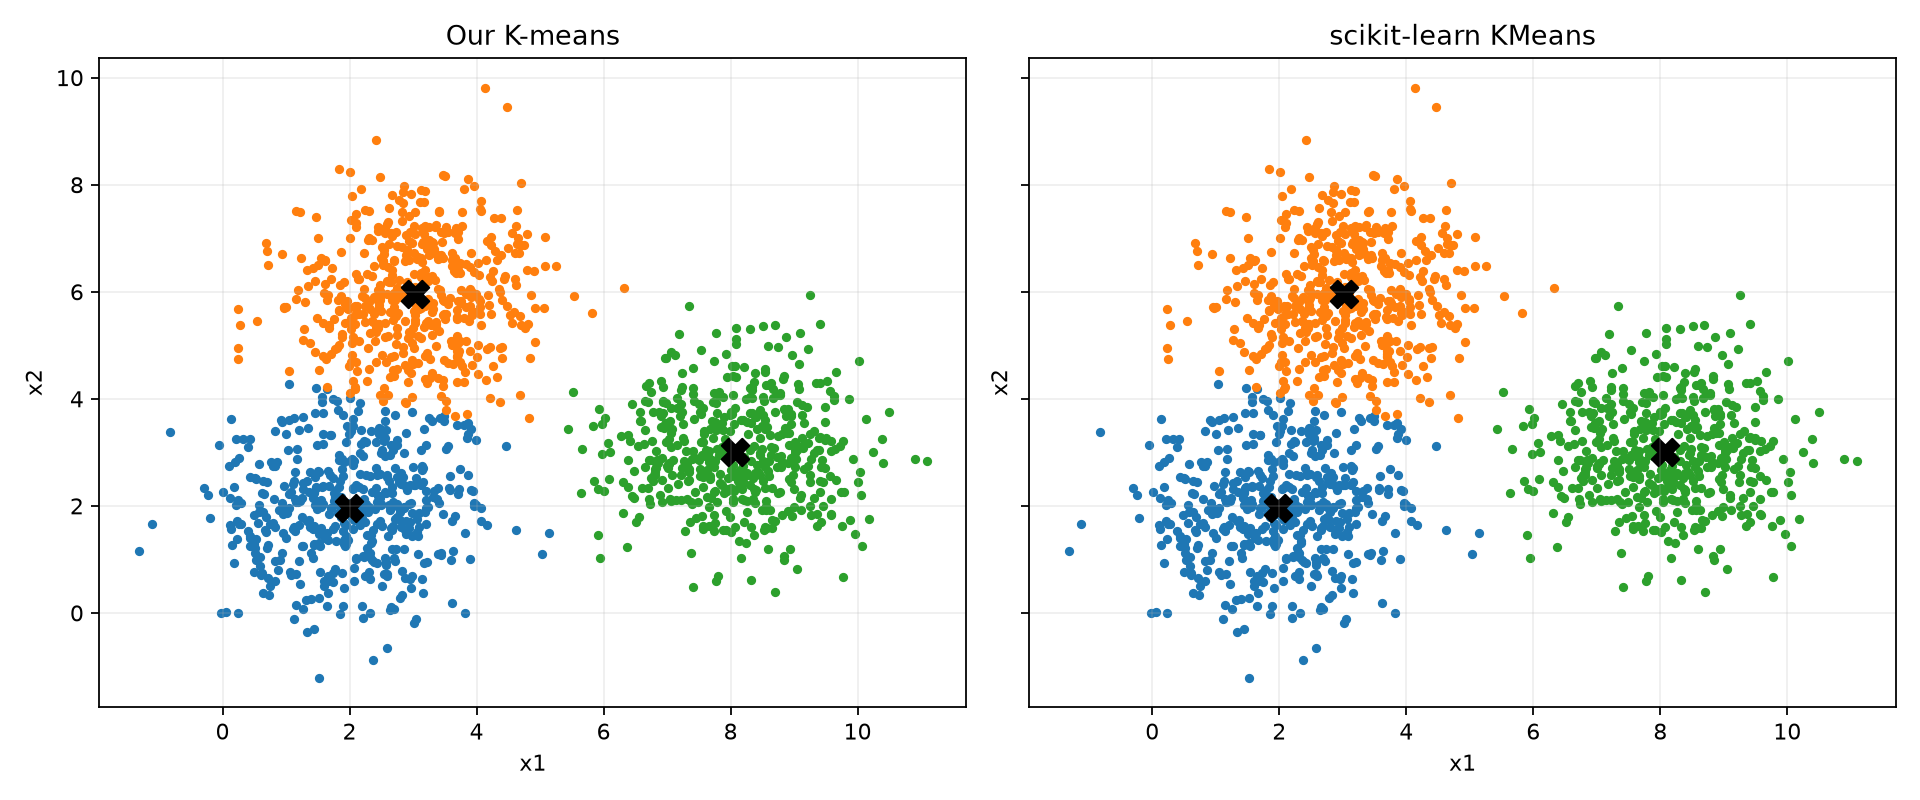
\includegraphics[width=0.98\textwidth]{kmeans_scikit_comparison.png}
    \caption{So sánh trực quan kết quả tự cài đặt (trái) và Scikit-learn (phải):
    màu thể hiện nhãn cụm đã ghép, dấu X là tâm cụm.}
    \label{fig:kmeans-comparison}
\end{figure}

Hình~\ref{fig:kmeans-comparison} cho thấy hai cách cho cùng cách chia ba vùng
dữ liệu và các tâm nằm ở cùng vị trí. Đây là kiểm tra trực quan phù hợp với
kết quả khớp nhãn và inertia ở trên.
